\section{Skewness}
Veri dağılımının simetrisini ve asimetrisini ölçen bir istatistiksel terimdir.. Üç tür çarpıklık vardır:

\begin{itemize}
    \item \textbf{Negatif (sol) çarpıklık:} Sola doğru çarpık, kuyruk sağ tarafta daha uzundur. Veri setindeki büyük değerler daha sık görülürken küçük değerler daha az sıklıkta görülür. Mean < Median < Mode.
    \item \textbf{Pozitif (sağ) çarpıklık:} Sağa doğru çarpık, kuyruk sol tarafta daha uzundur. Veri setindeki küçük değerler daha sık görülürken büyük değerler daha az sıklıkta görülür. Mode < Median < Mean.
    \item \textbf{Simetrik dağılım:} Çarpıklık yok. Veri setindeki büyük ve küçük değerlerin görülme sıklığı eşittir.
\end{itemize}

\begin{figure}[h]
    \centering
    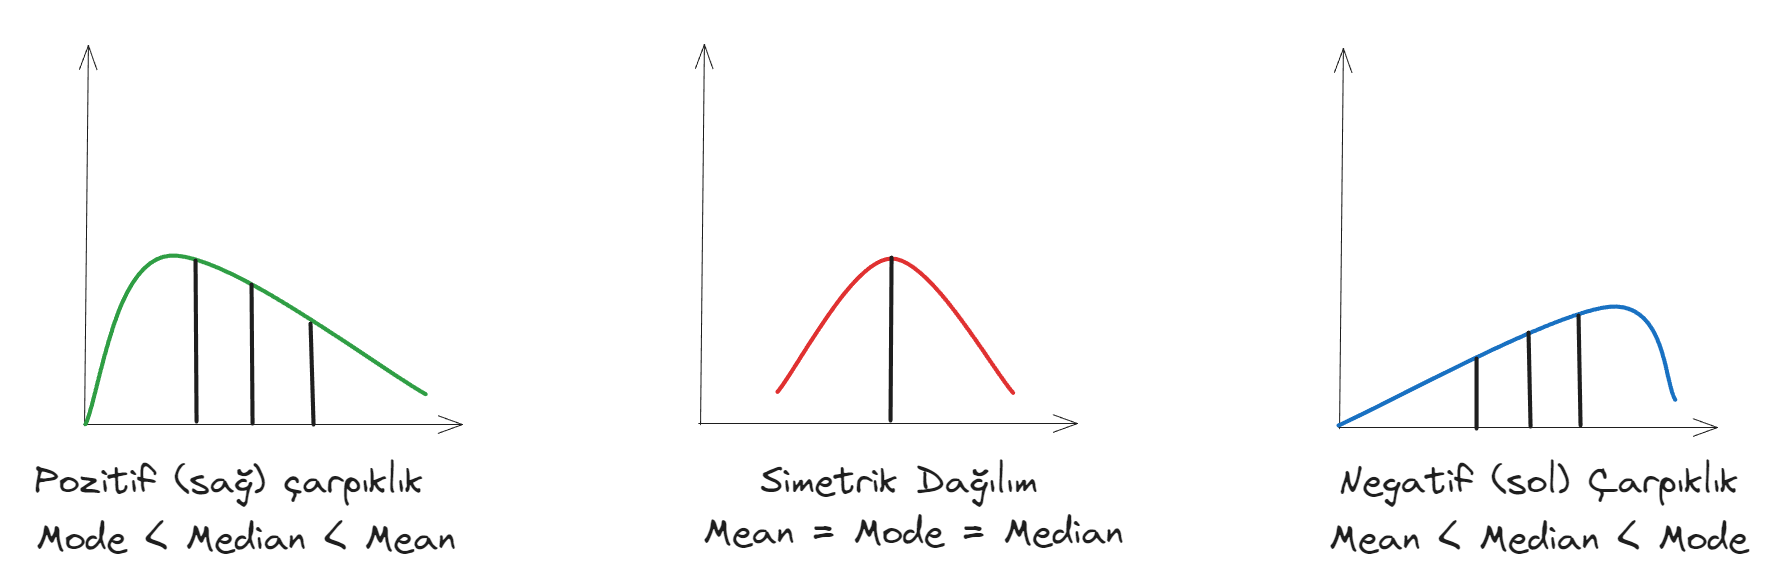
\includegraphics[width=1\textwidth]{images/skewness_types.png}
    \caption{Çarpıklık türleri.}
    \label{fig:enter-label}
\end{figure}

Skewness, veri setindeki örneklem gözlemlerinin üçüncü merkezi momentine dayanır. Veri setindeki her bir özellik için skewness hesaplamak için genellikle şu formül kullanılır:

\[\text{Skewness} = \frac{\sum_{i=1}^{n} (x_i - \bar{x})^3}{n \cdot s^3}\]



\subsection{Box-Cox Dönüşümü}
Veri setindeki çarpıklığı azaltmak veya veriyi normal dağılıma yakın bir hale getirmek için kullanılır. lambda parametresi belirlenerek gerçekleştirilir.

\[y(\lambda) = \begin{cases} \frac{{y^\lambda - 1}}{{\lambda}}, & \text{if } \lambda \neq 0, \\ \log(y), & \text{if } \lambda = 0. \end{cases}\]

\begin{lstlisting}[language=Python]
from scipy.stats import boxcox

train, test = train_test_split(df, test_size=0.2)
train, fitted_lambda = boxcox(train)
test = boxcox(test, fitted_lambda)
\end{lstlisting}

\newpage